\documentclass[12pt,t]{beamer}
\subtitle{09 -- Weighted Graphs}
\newcommand{\shorttitle}{Weighted Graphs}
\usepackage{graphicx}
\setbeameroption{hide notes}
\setbeamertemplate{note page}[plain]

% get rid of junk
\usetheme{default}
\beamertemplatenavigationsymbolsempty
\hypersetup{pdfpagemode=UseNone} % don't show bookmarks on initial view

% font
\usepackage{fontspec}
\setsansfont{TeX Gyre Heros}
\setbeamerfont{note page}{family*=pplx,size=\footnotesize} % Palatino for notes
% "TeX Gyre Heros can be used as a replacement for Helvetica"
% In Unix, unzip the following into ~/.fonts
% In Mac, unzip it, double-click the .otf files, and install using "FontBook"
%   http://www.gust.org.pl/projects/e-foundry/tex-gyre/heros/qhv2.004otf.zip

% named colors
\definecolor{offwhite}{RGB}{249,242,215}
% \definecolor{foreground}{RGB}{255,255,255}
\definecolor{foreground}{RGB}{0,0,0}
% \definecolor{background}{RGB}{24,24,24}
\definecolor{background}{RGB}{255,255,255}
\definecolor{title}{RGB}{107,174,214}
\definecolor{gray}{RGB}{100,100,100}
\definecolor{subtitle}{RGB}{102,155,204}
\definecolor{hilight}{RGB}{20,180,204}
\definecolor{vhilight}{RGB}{255,111,207}
\definecolor{lolight}{RGB}{155,155,155}
%\definecolor{green}{RGB}{125,250,125}

% use those colors
\setbeamercolor{titlelike}{fg=title}
\setbeamercolor{subtitle}{fg=subtitle}
\setbeamercolor{institute}{fg=gray}
\setbeamercolor{normal text}{fg=foreground,bg=background}
\setbeamercolor{item}{fg=foreground} % color of bullets
\setbeamercolor{subitem}{fg=gray}
\setbeamercolor{itemize/enumerate subbody}{fg=gray}
\setbeamertemplate{itemize subitem}{{\textendash}}
\setbeamerfont{itemize/enumerate subbody}{size=\footnotesize}
\setbeamerfont{itemize/enumerate subitem}{size=\footnotesize}

% settings for table of contents
\setbeamercolor{section in toc}{fg=foreground,bg=background}
\setbeamerfont{subsection in toc}{size=\footnotesize}
\setbeamertemplate{section in toc}{{\scriptsize\leavevmode\raise1.35pt\hbox{$\blacktriangleright$}} \inserttocsection}
%\setbeamertemplate{subsection in toc}{\quad{\tiny\leavevmode\raise1.5pt\hbox{$\blacktriangleright$}} \footnotesize\inserttocsubsection\\}
\setbeamertemplate{subsection in toc}{\quad\quad\textendash\enspace\inserttocsubsection\\}

% page number
\setbeamertemplate{footline}{%
    \raisebox{5pt}{\makebox[\paperwidth]{\hfill\makebox[20pt]{\color{gray}
          \scriptsize\insertframenumber}}}\hspace*{5pt}}

% add a bit of space at the top of the notes page
\addtobeamertemplate{note page}{\setlength{\parskip}{12pt}}

% add subsection as frame title when it is empty
\makeatletter
  \CheckCommand*\beamer@checkframetitle{%
    \@ifnextchar\bgroup\beamer@inlineframetitle{}}
  \renewcommand*\beamer@checkframetitle{%
    \global\let\beamer@frametitle\relax\@ifnextchar%
    \bgroup\beamer@inlineframetitle{}}
\makeatother

\addtobeamertemplate{frametitle}{
  \ifx\insertframetitle\empty
      \frametitle{\insertsubsectionhead}
  \else
  \fi
 }{}


\usepackage{pbox}

% a few macros
\newcommand{\bi}{\begin{itemize}}
\newcommand{\ei}{\end{itemize}}
\newcommand{\ig}{\includegraphics}
\newcommand{\subt}[1]{{\footnotesize \color{subtitle} {#1}}}

% title info
\title{Kompetitives Programmieren}
%\author{Gregor Behnke}
\institute{Prof. Dr. Susanne Biundo-Stephan \\ Gregor Behnke \\ Institute of Artificial Intelligence\\ Ulm University}
\date{\tiny based on Bjarki Ágúst Guðmundsson's and Tómas Ken Magnússon's\\Competitive Programming}


\setbeamertemplate{footline}[text line]{%
  \parbox{\linewidth}{\vspace*{-8pt}\shorttitle \hfill \insertframenumber/\inserttotalframenumber}}
\setbeamertemplate{navigation symbols}{}


\newcommand{\specialcell}[2][c]{%
  \begin{tabular}[#1]{@{}c@{}}#2\end{tabular}}

% Tikz
\usepackage{tikz}
\usepackage{tkz-euclide}
\usetikzlibrary{arrows,shapes}
% \usepackage{intersections}
\usetkzobj{all}
\usetikzlibrary{arrows,shapes,angles,quotes,shapes, calc, decorations,matrix}
\usepackage{forest}
\pgfdeclarelayer{bg}    % declare background layer
\pgfsetlayers{bg,main}


% Minted
\usepackage{minted}
\usemintedstyle{tango}
\newminted{cpp}{fontsize=\footnotesize}

% Graph styles
\tikzstyle{vertex}=[circle,fill=black!50,minimum size=15pt,inner sep=0pt, font=\small]
\tikzstyle{selected vertex} = [vertex, fill=red!24]
\tikzstyle{selected2 vertex} = [vertex, fill=hilight!50, text=black]
\tikzstyle{vertex1} = [vertex, fill=red]
\tikzstyle{vertex2} = [vertex, fill=blue]
\tikzstyle{vertex3} = [vertex, fill=green, text=black]
\tikzstyle{vertex4} = [vertex, fill=yellow, text=black]
\tikzstyle{vertex5} = [vertex, fill=pink, text=black]
\tikzstyle{vertex6} = [vertex, fill=purple]
\tikzstyle{edge} = [draw,thick,-]
\tikzstyle{dedge} = [draw,thick,->]
\tikzstyle{weight} = [font=\scriptsize,pos=0.5]
\tikzstyle{selected edge} = [draw,line width=2pt,-,red!50]
\tikzstyle{ignored edge} = [draw,line width=5pt,-,black!20]


\begin{document}

% title slide
{
    \setbeamertemplate{footline}{} % no page number here
    \frame{
        \titlepage
    }
}






\begin{frame}{Today we're going to cover}
    \vspace{50pt}
    \bi
        \item Minimum spanning tree
        \item Shortest paths
        % \item Transitive closure
        % \item Minimax/maximin
       % \item Some known graph problems
        \item Maximum flow
      
        % - Minimum spanning tree (and variants)
        % - Shortest path (Dijkstra, Bellman-Ford, Floyd-Warshall)
        % - Transitive closure
        % - Minimax and maximin
        % - Special graphs
        %     - Trees
        %     - DAGs
        %     - Bipartite graphs
    \ei
\end{frame}

% TODO: ...

\begin{frame}{Weighted graphs}
    \vspace{30pt}
    \bi
        \item Now the edges in our graphs may have weights, which could represent
            \bi
                \item the distance of the road represented by the edge
                \item the cost of going over the edge
                \item some capacity of the edge
            \ei

        \item We can use a modified adjacency list to represent weighted graphs
    \ei
\end{frame}

\begin{frame}[fragile]{Weighted graphs}
    \begin{columns}[T]
        \begin{column}{.4\textwidth}
            \begin{minted}[fontsize=\footnotesize]{cpp}
struct edge {
    int u, v;
    int weight;

    edge(int _u, int _v, int _w) {
        u = _u;
        v = _v;
        weight = _w;
    }
};
            \end{minted}
        \end{column}%
        \hfill%
        \begin{column}{.6\textwidth}
            \begin{figure}
                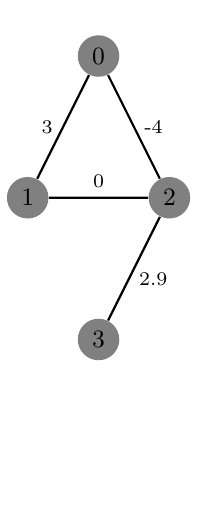
\begin{tikzpicture}[scale=1.8,auto,swap]
                    \node[vertex] (0) at (0.5,3) {0};
                    \node[vertex] (1) at (0,2) {1};
                    \node[vertex] (2) at (1,2) {2};
                    \node[vertex] (3) at (0.5,1) {3};

                    \path[edge] (0) -- node[weight,left] {3} (1);
                    \path[edge] (0) -- node[weight,right] {-4} (2);
                    \path[edge] (1) -- node[weight,above] {0} (2);
                    \path[edge] (2) -- node[weight,right,pos=0.6] {2.9} (3);

                    \pgfresetboundingbox
                    \path [use as bounding box] (0,0) rectangle (1,3.2);
                \end{tikzpicture}
            \end{figure}
        \end{column}%
    \end{columns}
\end{frame}

\begin{frame}[fragile]{Weighted graphs}
    \begin{columns}[T]
        \begin{column}{.4\textwidth}
            \begin{minted}[fontsize=\footnotesize]{cpp}
vector<edge> adj[4];

adj[0].push_back(edge(0, 1, 3));
adj[0].push_back(edge(0, 2, -4));

adj[1].push_back(edge(1, 0, 3));
adj[1].push_back(edge(1, 2, 0));

adj[2].push_back(edge(2, 0, -4));
adj[2].push_back(edge(2, 1, 0));
adj[2].push_back(edge(2, 3, 2.9));

adj[3].push_back(edge(3, 2, 2.9));

            \end{minted}
        \end{column}%
        \hfill%
        \begin{column}{.6\textwidth}
            \begin{figure}
                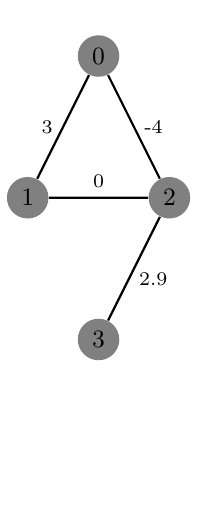
\begin{tikzpicture}[scale=1.8,auto,swap]
                    \node[vertex] (0) at (0.5,3) {0};
                    \node[vertex] (1) at (0,2) {1};
                    \node[vertex] (2) at (1,2) {2};
                    \node[vertex] (3) at (0.5,1) {3};

                    \path[edge] (0) -- node[weight,left] {3} (1);
                    \path[edge] (0) -- node[weight,right] {-4} (2);
                    \path[edge] (1) -- node[weight,above] {0} (2);
                    \path[edge] (2) -- node[weight,right,pos=0.6] {2.9} (3);

                    \pgfresetboundingbox
                    \path [use as bounding box] (0,0) rectangle (1,3.2);
                \end{tikzpicture}
            \end{figure}
        \end{column}%
    \end{columns}
\end{frame}

\begin{frame}[fragile]{Weighted graphs}
    \begin{columns}[T]
        \begin{column}{.4\textwidth}
            \begin{minted}[fontsize=\footnotesize]{cpp}
vi adj[4];
vi w[4];

adj[0].push_back(1); w[0].push_back(3);
adj[0].push_back(2); w[0].push_back(-4);

adj[1].push_back(0); w[1].push_back(3);
adj[1].push_back(2); w[1].push_back(0);

adj[2].push_back(0); w[2].push_back(-4);
adj[2].push_back(1); w[2].push_back(0);
adj[2].push_back(3); w[2].push_back(2.9);

adj[3].push_back(2); w[3].push_back(2.9);

            \end{minted}
        \end{column}%
        \hfill%
        \begin{column}{.6\textwidth}
            \begin{figure}
                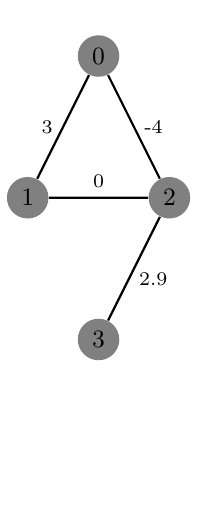
\begin{tikzpicture}[scale=1.8,auto,swap]
                    \node[vertex] (0) at (0.5,3) {0};
                    \node[vertex] (1) at (0,2) {1};
                    \node[vertex] (2) at (1,2) {2};
                    \node[vertex] (3) at (0.5,1) {3};

                    \path[edge] (0) -- node[weight,left] {3} (1);
                    \path[edge] (0) -- node[weight,right] {-4} (2);
                    \path[edge] (1) -- node[weight,above] {0} (2);
                    \path[edge] (2) -- node[weight,right,pos=0.6] {2.9} (3);

                    \pgfresetboundingbox
                    \path [use as bounding box] (0,0) rectangle (1,3.2);
                \end{tikzpicture}
            \end{figure}
        \end{column}%
    \end{columns}
\end{frame}


\begin{frame}{Minimum spanning tree}
    \vspace{20pt}
    \bi
        \item We have an undirected weighted graph
        \item The vertices along with a subset of the edges in the graph is called a spanning tree if
            \bi
                \item it forms a tree (i.e.\ does not contain a cycle) and
                \item the tree spans all vertices (all vertices can reach all other vertices)
            \ei
        \vspace{10pt}
        \item The weight of a spanning tree is the sum of the weights of the edges in the subset
        \vspace{10pt}
        \item We want to find a minimum spannig tree
    \ei
\end{frame}

\begin{frame}{Minimum spanning tree}
    \vspace{20pt}
    \bi
        \item Several greedy algorithms work
        \vspace{10pt}
        \item Go through the edges in the graph in increasing order of weight
        \item Greedily pick an edge if it doesn't form a cycle (Union-Find can be used to keep track of when we would get a cycle)
        \item When we've gone through all edges, we have a minimum spanning tree
        \vspace{10pt}
        \item This is Kruskal's algorithm
        \item Time complexity is $O(E \log E)$
    \ei
\end{frame}

\begin{frame}[fragile]{Minimum spanning tree}
    \begin{minted}[fontsize=\scriptsize]{cpp}

bool edge_cmp(const edge &a, const edge &b) {
    return a.weight < b.weight;
}

vector<edge> mst(int n, vector<edge> edges) {
    union_find uf(n);
    sort(edges.begin(), edges.end(), edge_cmp);

    vector<edge> res;
    FORIT(e,edges) if (uf.find(e->u) != uf.find(e->v)) {
        uf.unite(e->u, e->v);
        res.push_back(*e);
    }

    return res;
}
    \end{minted}
\end{frame}

% TODO: Example problem: 
% \begin{frame}{Example problem: Dark roads}
%     \bi
%         \item http://uva.onlinejudge.org/external/116/11631.html
%     \ei
% \end{frame}

\begin{frame}{Shortest paths}
    \vspace{40pt}
    \bi
        \item We have a weighted graph (undirected or directed)
        \item Given two vertices $u,v$, what is the shortest path from $u$ to $v$?
        \vspace{10pt}
        \item If all weights are the same, this can be solved with breadth-first search
        \item Of course, this is usually not the case...
    \ei
\end{frame}

\begin{frame}{Shortest paths}
    \vspace{40pt}
    \bi
        \item There are many known algorithms to find shortest paths
        \item Like breadth-first search, these algorithms usually find the shortest paths from a given start vertex to all other vertices
        \vspace{5pt}
        \item Let's take a quick look at Dijkstra's algorithm, the Bellman-Ford algorithm, and the Floyd-Warshall algorithm
    \ei
\end{frame}

% TODO: Dijkstra's algorithm
% \begin{frame}{Dijkstra's algorithm}
%     \bi
%         \item 
%     \ei
% \end{frame}

\begin{frame}[fragile]{Dijkstra's algorithm}
    \begin{minted}[fontsize=\scriptsize]{cpp}
vector<edge> adj[1000];
int dist[1000];

void dijkstra(int start) {
    FOR(i,0,1000) dist[i] = oo;
    dist[start] = 0;
    
    priority_queue<pii, vector<pii>, greater<pii> > pq;
    pq.push(make_pair(dist[start], start));

    while (!pq.empty()) {
        int u = pq.top().second;
        pq.pop();

        FORIT(i,adj[u]) if (i->weight + dist[u] < dist[i->v]) {
            dist[i->v] = i->weight + dist[u];
            pq.push(make_pair(dist[i->v], i->v));
        }
    }
}
    \end{minted}
\end{frame}

\begin{frame}[fragile]{Dijkstra's algorithm}
    \begin{minted}[fontsize=\scriptsize]{cpp}
vector<edge> adj[1000];
int dist[1000];

void dijkstra(int start) {
    FOR(i,0,1000) dist[i] = oo;
    dist[start] = 0;
    
    priority_queue<pii> pq;
    pq.push(make_pair(-dist[start], start));

    while (!pq.empty()) {
        int u = pq.top().second;
        pq.pop();

        FORIT(i,adj[u]) if (i->weight + dist[u] < dist[i->v]) {
            dist[i->v] = i->weight + dist[u];
            pq.push(make_pair(-dist[i->v], i->v));
        }
    }
}
    \end{minted}
\end{frame}

\begin{frame}{Dijkstra's algorithm}
    \vspace{50pt}
    \bi
        \item Time complexity is $O(V \log E)$
        \vspace{10pt}
        \item Note that this only works for non-negative weights
    \ei
\end{frame}

% TODO: Bellman-Ford algorithm
\begin{frame}[fragile]{Bellman-Ford algorithm}
    \begin{minted}[fontsize=\footnotesize]{cpp}
void bellman_ford(int n, int start) {
    dist[start] = 0;
    FOR(round,0,n-1) FOR(u,0,n) FORIT(e, adj[u])
        dist[e->v] = min(dist[e->v], e->weight + dist[u]);
}
    \end{minted}
\end{frame}

\begin{frame}{Bellman-Ford algorithm}
    \vspace{50pt}
    \bi
        \item Time complexity is $O(V\times E)$
        \vspace{10pt}
        \item Can be used to detect negative-weight cycles
    \ei
\end{frame}

% TODO: Floyd-Warshall algorithm
\begin{frame}{Floyd-Warshall algorithm}
    \vspace{20pt}
    \bi
        \item What about using dynamic programming to compute shortest paths?
        \vspace{10pt}
    \item Let $\mathrm{sp}(k, i, j)$ be the shortest path from $i$ to $j$ if we're only allowed to travel through the vertices $0$, \ldots, $k$
        \vspace{5pt}
    \item Base case: $\mathrm{sp}(k, i, j) = 0$ if $i = j$
    \item Base case: $\mathrm{sp}(-1, i, j) = \mathrm{weight}[a][b]$ if $(i,j) \in E$
    \item Base case: $\mathrm{sp}(-1, i, j) = \infty$
        \vspace{5pt}
    \item $\mathrm{sp}(k, i, j) = \mathrm{min} \left\{
	\begin{array}{l}
        \mathrm{sp}(k - 1, i, k) + \mathrm{sp}(k - 1, k, j) \\
        \mathrm{sp}(k - 1, i, j)
	\end{array}
\right.$
    \ei
\end{frame}

\begin{frame}[fragile]{Floyd-Warshall algorithm}
    \begin{minted}[fontsize=\scriptsize]{cpp}
int dist[1000][1000];
int weight[1000][1000];

void floyd_warshall(int n) {
    FOR(i,0,n) FOR(j,0,n) dist[i][j] = i == j ? 0 : weight[i][j];

    FOR(k,0,n) FOR(i,0,n) FOR(j,0,n)
        dist[i][j] = min(dist[i][j], dist[i][k] + dist[k][j]);
}
    \end{minted}
\end{frame}

\begin{frame}{Floyd-Warshall algorithm}
    \vspace{40pt}
    \bi
\item Computes all-pairs shortest paths
\item Time complexity is clearly $O(n^3)$
\item Very simple to code
    \vspace{10pt}
\item Can also be used backwards to remove transitive edges
    \ei
\end{frame}

\begin{frame}{Maximum Flow}
    \bi
\item Given a weighted graph $G = (V,E,c)$, two vertices $s,t$ and a capacity function $c$
\item How much can be ''transported'' from $s$ to $t$?
\item Solution is a flow function $f : E \rightarrow \mathbb R_{\geq 0}$ where
  \bi
    \item $c((u,v)) \geq f((u,v)) \quad \quad\quad\quad \quad \forall (u,v) \in E$
    \item $\sum_uf((u,v)) = \sum_uf((v,u)) \quad \quad \forall u \in V \setminus\{s,t\}$
  \ei
  \item Find a flow $f$ such that $\sum_v f((s,v))$ is maximal
  \vspace{10pt} \pause
  \item Min-cut:
  \bi
    \item Find a subset $C'\subseteq E$ with minimum weight (summed capacity) such that $s$ and $t$ are not connected any more
  \ei
  \vspace{10pt} \pause
  \item Max-Flow = Min-Cut
    \ei
\end{frame}

\begin{frame}{Maximum Flow}
  \begin{figure}
                \begin{tikzpicture}[scale=1.8,auto,swap]
                    \node[vertex] (s) at (0,2) {s};
                    \node[vertex] (t) at (4,2) {t};
                    \node[vertex] (1) at (1,3) {1};
                    \node[vertex] (2) at (1,1) {2};
                    \node[vertex] (3) at (2,2) {3};
                    \node[vertex] (4) at (3,3) {4};
                    \node[vertex] (5) at (3,1) {5};

                    \path[edge,->] (s) -- node[weight,left] {\only<2->{1/}2} (1);
                    \path[edge,->] (s) -- node[weight,left] {\only<2->{4/}6} (2);
                    \path[edge,->] (1) -- node[weight,right] {\only<2->{1/}1} (3);
                    \path[edge,->] (2) -- node[weight,right] {\only<2->{2/}3} (3);
                    \path[edge,->] (2) -- node[weight,above] {\only<2->{2/}4} (5);
                    \only<-2>{\path[edge,->] (3) -- node[weight,left] {\only<2->{3/}3} (4);}
                    \only<3->{\path[selected edge,->] (3) -- node[weight,left] {\only<2->{3/}3} (4);}
                    \path[edge,->] (3) -- node[weight,left] {\only<2->{0/}3} (5);
                    \path[edge,->] (4) -- node[weight,right] {\only<2->{3/}5} (t);
                    \only<-2>{\path[edge,->] (5) -- node[weight,right] {\only<2->{2/}2} (t);}
                    \only<3->{\path[selected edge,->] (5) -- node[weight,right] {\only<2->{2/}2} (t);}

%                     \pgfresetboundingbox
%                     \path [use as bounding box] (0,0) rectangle (1,3.2);
                \end{tikzpicture}
            \end{figure}
       \bi
	\item<4-> A Min-Cut can be found by DFS
	\bi
	  \item<5-> Any edge $e$ with $c(e) = f(e)$ is in the cut
	  \item<5-> Don't traverse these edges
	\ei
       \ei
\end{frame}



\begin{frame}{How to compute a Maximum Flow}
       \bi
	\item Start with $f(e) = 0$ and successively add more flow
	\item Decisions to increase the flow can be wrong
	\item[$\rightarrow$] Augmenting paths in the residual graph
       \ei

  \begin{figure}
                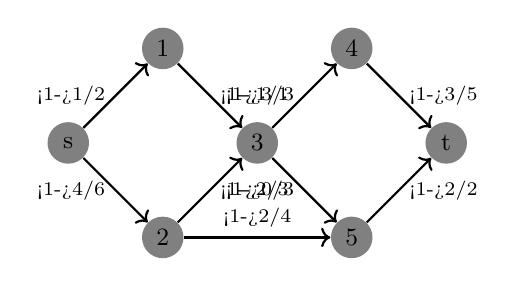
\begin{tikzpicture}[scale=1.2,auto,swap]
                    \node[vertex] (s) at (0,2) {s};
                    \node[vertex] (t) at (4,2) {t};
                    \node[vertex] (1) at (1,3) {1};
                    \node[vertex] (2) at (1,1) {2};
                    \node[vertex] (3) at (2,2) {3};
                    \node[vertex] (4) at (3,3) {4};
                    \node[vertex] (5) at (3,1) {5};

                    \path[edge,->] (s) -- node[weight,left] {\only<1->{1/}2} (1);
                    \path[edge,->] (s) -- node[weight,left] {\only<1->{4/}6} (2);
                    \path[edge,->] (1) -- node[weight,right] {\only<1->{1/}1} (3);
                    \path[edge,->] (2) -- node[weight,right] {\only<1->{2/}3} (3);
                    \path[edge,->] (2) -- node[weight,above] {\only<1->{2/}4} (5);
                    \path[edge,->] (3) -- node[weight,left] {\only<1->{3/}3} (4);
                    \path[edge,->] (3) -- node[weight,left] {\only<1->{0/}3} (5);
                    \path[edge,->] (4) -- node[weight,right] {\only<1->{3/}5} (t);
                    \path[edge,->] (5) -- node[weight,right] {\only<1->{2/}2} (t);
                \end{tikzpicture}
            \end{figure}
            \begin{figure}
                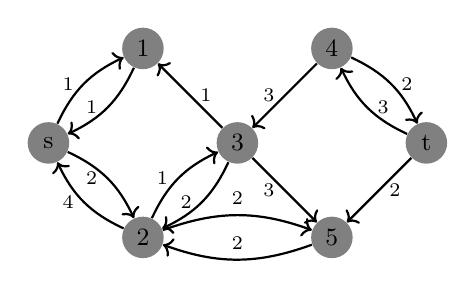
\begin{tikzpicture}[scale=1.2,auto,swap]
                    \node[vertex] (s) at (0,2) {s};
                    \node[vertex] (t) at (4,2) {t};
                    \node[vertex] (1) at (1,3) {1};
                    \node[vertex] (2) at (1,1) {2};
                    \node[vertex] (3) at (2,2) {3};
                    \node[vertex] (4) at (3,3) {4};
                    \node[vertex] (5) at (3,1) {5};

                    \path[edge,->] (s) edge[bend left=20] node[weight, left] {1} (1);
                    \path[edge,->] (1) edge[bend right=-20] node[weight, left] {1} (s);

                    \path[edge,->] (s) edge[bend left=20] node[weight,left] {2} (2);
                    \path[edge,->] (2) edge[bend right=-20] node[weight,left] {4} (s);

                    \path[edge,->] (3) -- node[weight,right] {1} (1);

                    \path[edge,->] (2) edge[bend left=20] node[weight,left] {1} (3);
                    \path[edge,->] (3) edge[bend right=-20] node[weight,left] {2} (2);

                    \path[edge,->] (2) edge[bend left=20] node[weight,above] {2} (5);
                    \path[edge,->] (5) edge[bend right=-20] node[weight,above] {2} (2);

                    \path[edge,->] (4) -- node[weight,left] {3} (3);
                    \path[edge,->] (3) -- node[weight,left] {3} (5);

                    \path[edge,->] (4) edge[bend left=20] node[weight,right] {2} (t);
                    \path[edge,->] (t) edge[bend right=-20] node[weight,right] {3} (4);

                    \path[edge,->] (t) -- node[weight,right] {2} (5);
                \end{tikzpicture}
            \end{figure}
\end{frame}


\begin{frame}{How to compute a Maximum Flow}
  \begin{figure}
                \begin{tikzpicture}[scale=1.2,auto,swap]
                    \node[vertex] (s) at (0,2) {s};
                    \node[vertex] (t) at (4,2) {t};
                    \node[vertex] (1) at (1,3) {1};
                    \node[vertex] (2) at (1,1) {2};
                    \node[vertex] (3) at (2,2) {3};
                    \node[vertex] (4) at (3,3) {4};
                    \node[vertex] (5) at (3,1) {5};

                    \path[edge,->] (s) -- node[weight,left] {\only<1-8>{0/}\only<9->{1/}2} (1);
                    \path[edge,->] (s) -- node[weight,left] {\only<1-2>{0/}\only<3-5>{2/}\only<6->{4/}6} (2);
                    \path[edge,->] (1) -- node[weight,right] {\only<1-8>{0/}\only<9->{1/}1} (3);
                    \path[edge,->] (2) -- node[weight,right] {\only<1-2>{0/}\only<3->{2/}3} (3);
                    \path[edge,->] (2) -- node[weight,above] {\only<1-5>{0/}\only<6->{2/}4} (5);
                    \path[edge,->] (3) -- node[weight,left] {\only<1-5>{0/}\only<6-8>{2/}\only<9->{3/}3} (4);
                    \path[edge,->] (3) -- node[weight,left] {\only<1-2>{0/}\only<3-5>{2/}\only<6->{0/}3} (5);
                    \path[edge,->] (4) -- node[weight,right] {\only<1-5>{0/}\only<6-8>{2/}\only<9->{3/}5} (t);
                    \path[edge,->] (5) -- node[weight,right] {\only<1-2>{0/}\only<3->{2/}2} (t);
                \end{tikzpicture}
            \end{figure}
            \only<1-9>{\begin{figure}
                \begin{tikzpicture}[scale=1.2,auto,swap]
                    \node[vertex] (s) at (0,2) {s};
                    \node[vertex] (t) at (4,2) {t};
                    \node[vertex] (1) at (1,3) {1};
                    \node[vertex] (2) at (1,1) {2};
                    \node[vertex] (3) at (2,2) {3};
                    \node[vertex] (4) at (3,3) {4};
                    \node[vertex] (5) at (3,1) {5};

                    \only<-7>{\path[edge,->] (s) -- node[weight,left] {2} (1);}
                    \only<8-9>{\path[selected edge,->] (s) -- node[weight,left] {2} (1);}

                    \only<-1>{\path[edge,->] (s) -- node[weight,left] {6} (2);}
                    \only<2-3>{\path[selected edge,->] (s) -- node[weight,left] {6} (2);}
                    \only<4>{\path[edge,->] (s) edge[bend left=20] node[weight,left] {4} (2);}
                    \only<4-6>{\path[edge,->] (2) edge[bend right=-20] node[weight,left] {2} (s);}
                    \only<5-6>{\path[selected edge,->] (s) edge[bend left=20] node[weight,left] {4} (2);}
                    \only<7->{\path[edge,->] (s) edge[bend left=20] node[weight,left] {2} (2);}
                    \only<7->{\path[edge,->] (2) edge[bend right=-20] node[weight,left] {4} (s);}
                    
                    \only<-7>{\path[edge,->] (1) -- node[weight,right] {1} (3);}
                    \only<8-9>{\path[selected edge,->] (1) -- node[weight,right] {1} (3);}

                    \only<-1>{\path[edge,->] (2) -- node[weight,left] {3} (3);}
                    \only<2-3>{\path[selected edge,->] (2) -- node[weight,left] {3} (3);}
                    \only<4->{\path[edge,->] (2) edge[bend left=20] node[weight,left] {1} (3);}
                    \only<4->{\path[edge,->] (3) edge[bend right=-20] node[weight,left] {2} (2);}
                    
                    \only<-4>{\path[edge,->] (2) -- node[weight,above] {4} (5);}
                    \only<5-6>{\path[selected edge,->] (2) -- node[weight,above] {4} (5);}
                    \only<7->{\path[edge,->] (2) edge[bend left=20] node[weight,above] {2} (5);}
                    \only<7->{\path[edge,->] (5) edge[bend right=-20] node[weight,above] {2} (2);}
                    
                    \only<-4>{ \path[edge,->] (3) -- node[weight,left] {3} (4);}
                    \only<5-6>{ \path[selected edge,->] (3) -- node[weight,left] {3} (4);}
                    \only<7>{ \path[edge,->] (3) edge[bend left=20] node[weight,left] {1} (4);}
                    \only<7->{ \path[edge,->] (4) edge[bend right=-20] node[weight,left] {2} (3);}
                    \only<8-9>{ \path[selected edge,->] (3) edge[bend left=20] node[weight,left] {1} (4);}
                    
                    \only<-1>{\path[edge,->] (3) -- node[weight,left] {3} (5);}
                    \only<2-3>{\path[selected edge,->] (3) -- node[weight,left] {3} (5);}
                    \only<4-6>{\path[edge,->] (3) edge[bend left=20] node[weight,left] {1} (5);}
                    \only<4>{\path[edge,->] (5) edge[bend right=-20] node[weight,left] {2} (3);}
                    \only<5-6>{\path[selected edge,->] (5) edge[bend right=-20] node[weight,left] {2} (3);}
                    \only<7->{\path[edge,->] (3) -- node[weight,left] {3} (5);}
                    
                    \only<-4>{\path[edge,->] (4) -- node[weight,right] {5} (t);}
                    \only<5-6>{\path[selected edge,->] (4) -- node[weight,right] {5} (t);}
                    \only<7>{\path[edge,->] (4) edge[bend left=20] node[weight,right] {3} (t);}
                    \only<7->{\path[edge,->] (t) edge[bend right=-20] node[weight,right] {2} (4);}
                    \only<8-9>{\path[selected edge,->] (4) edge[bend left=20] node[weight,right] {3} (t);}
                    
                    \only<-1>{\path[edge,->] (5) -- node[weight,right] {2} (t);}
                    \only<2-3>{\path[selected edge,->] (5) -- node[weight,right] {2} (t);}
                    \only<4->{\path[edge,->] (t) -- node[weight,right] {2} (5);}
                \end{tikzpicture}
            \end{figure}}
            \only<10>{ \begin{figure}
                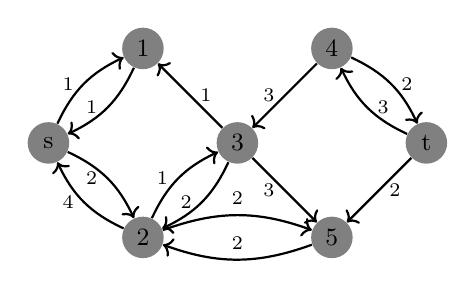
\begin{tikzpicture}[scale=1.2,auto,swap]
                    \node[vertex] (s) at (0,2) {s};
                    \node[vertex] (t) at (4,2) {t};
                    \node[vertex] (1) at (1,3) {1};
                    \node[vertex] (2) at (1,1) {2};
                    \node[vertex] (3) at (2,2) {3};
                    \node[vertex] (4) at (3,3) {4};
                    \node[vertex] (5) at (3,1) {5};

                    \path[edge,->] (s) edge[bend left=20] node[weight, left] {1} (1);
                    \path[edge,->] (1) edge[bend right=-20] node[weight, left] {1} (s);

                    \path[edge,->] (s) edge[bend left=20] node[weight,left] {2} (2);
                    \path[edge,->] (2) edge[bend right=-20] node[weight,left] {4} (s);

                    \path[edge,->] (3) -- node[weight,right] {1} (1);

                    \path[edge,->] (2) edge[bend left=20] node[weight,left] {1} (3);
                    \path[edge,->] (3) edge[bend right=-20] node[weight,left] {2} (2);

                    \path[edge,->] (2) edge[bend left=20] node[weight,above] {2} (5);
                    \path[edge,->] (5) edge[bend right=-20] node[weight,above] {2} (2);

                    \path[edge,->] (4) -- node[weight,left] {3} (3);
                    \path[edge,->] (3) -- node[weight,left] {3} (5);

                    \path[edge,->] (4) edge[bend left=20] node[weight,right] {2} (t);
                    \path[edge,->] (t) edge[bend right=-20] node[weight,right] {3} (4);

                    \path[edge,->] (t) -- node[weight,right] {2} (5);
                \end{tikzpicture}
            \end{figure}}
\end{frame}


\begin{frame}{Runtime}
       \bi
	\item Only efficient with additions
	\item E.g. use always use the shortest path from $s$ to $t$ $\rightarrow O(m^2n)$
	\item If all capacities are $1$ the runtime becomes $O(mn)$
	\vspace{10pt}
	\item There are better algorithms, like Push-Relable or Dinic
	\item Dinic computes \emph{Blocking Flows} ($\approx$ all shortest paths from $s$ to $t$). For graphs with capacity $1$ and $\min\{deg^+(v),deg^-(v)\} \leq 1$ for all vertices $v$ its runtime is $\mathcal O(m \sqrt{n})$
		\ei
\end{frame}

\begin{frame}{Modelling}
       \bi
	\item Multiple sources (sinks)?
	\item[$\rightarrow$] add a new artificial master source (sink)
	\vspace{10pt}
	\item Vertex capacities?
	\item[$\rightarrow$] split each vertex in two and connect them with edges having the node's capacity
	\vspace{10pt}
	\item The TCR also contains a version that computes the cost-minimal Max Flow and an algorithm for Maximum circulation
       \ei
\end{frame}

\begin{frame}{What to use Maximum Flow for?}
       \bi
	\item Sometimes it is ''obvious''
	\item There are some common applications
	\bi
	  \item Bipartite Matching
	  \item Disjoint Paths
	\ei
       \ei
\end{frame}

\begin{frame}{Bipartite Matching}
	\bi
		\item<3-> Max Flow $=$ Max Matching
	\ei
   \begin{figure}
                \begin{tikzpicture}[scale=1.2,auto,swap]
                    \node[vertex] (1) at (1,4) {1};
                    \node[vertex] (2) at (1,3) {2};
                    \node[vertex] (3) at (1,2) {3};
                    \node[vertex] (4) at (1,1) {4};
                    \node[vertex] (5) at (3,3) {5};
                    \node[vertex] (6) at (3,2) {6};
                    \node[vertex] (7) at (3,1) {7};

                    \only<3->{
                    	\node[vertex] (s) at (-1,2.5) {s};
	                    \node[vertex] (t) at (5,2) {t};
	                }

                    \path[edge] (1) -- node[weight,right] {} (5);
                    \only<1>{\path[edge] (2) -- node[weight,right] {} (5);}
                    \only<2>{\path[selected edge] (2) -- node[weight,right] {} (5);}
                    \path[edge] (2) -- node[weight,above] {} (6);
                    \only<1>{\path[edge] (3) -- node[weight,left] {} (6);}
                    \only<2>{\path[selected edge] (3) -- node[weight,left] {} (6);}
                    \path[edge] (3) -- node[weight,left] {} (7);
                    \only<1>{\path[edge] (4) -- node[weight,right] {} (7);}
                    \only<2>{\path[selected edge] (4) -- node[weight,right] {} (7);}
                    \path[edge] (4) -- node[weight,right] {} (6);


					\only<3->{
						\path[edge,->] (s) -- node[weight,right] {} (1);
						\path[edge,->] (s) -- node[weight,right] {} (2);
						\path[edge,->] (s) -- node[weight,right] {} (3);
						\path[edge,->] (s) -- node[weight,right] {} (4);
						
                    	\path[edge,->] (1) -- node[weight,right] {} (5);
                    	\path[edge,->] (2) -- node[weight,right] {} (5);
                    	\path[edge,->] (2) -- node[weight,above] {} (6);
                   		\path[edge,->] (3) -- node[weight,left] {} (6);
                   		\path[edge,->] (3) -- node[weight,left] {} (7);
                   		\path[edge,->] (4) -- node[weight,right] {} (7);
                    	\path[edge,->] (4) -- node[weight,right] {} (6);
                    	
                    	\path[edge,->] (5) -- node[weight,right] {} (t);
                    	\path[edge,->] (6) -- node[weight,right] {} (t);
                    	\path[edge,->] (7) -- node[weight,right] {} (t);
                    }

                \end{tikzpicture}
            \end{figure}      

       \bi
	\item<4> Simple reduction to Max Flow
	\item<4> Flow with unit capacities is faster than 
       \ei
\end{frame}

\begin{frame}{Disjoint paths}
       \bi
	\item Given a graph $G=(V,E)$ and two vertices $s$ and $t$.
	\item How many edge disjoint paths are there from $s$ to $t$?
       \ei
       \begin{figure}
                \begin{tikzpicture}[scale=1.2,auto,swap]
                    \node[vertex] (1) at (1,2.5) {1};
                    \node[vertex] (2) at (1,1.5) {2};
                    \node[vertex] (3) at (2,2.5) {3};
                    \node[vertex] (4) at (2,1.5) {4};
                    \node[vertex] (5) at (3,3) {5};
                    \node[vertex] (6) at (3,2) {6};
                    \node[vertex] (7) at (3,1) {7};
                  	\node[vertex] (s) at (-1,2) {s};
                    \node[vertex] (t) at (5,2) {t};

					%\only<1>{
                    %\path[edge] (s) -- node[weight,right] {} (1);
                    %\path[edge] (s) -- node[weight,right] {} (2);
                    %\path[edge] (s) -- node[weight,right] {} (6);
                    %\path[edge] (1) -- node[weight,right] {} (5);
                    %\path[edge] (1) -- node[weight,right] {} (3);
                    %\path[edge] (2) -- node[weight,right] {} (4);
                    %\path[edge] (3) -- node[weight,right] {} (5);
                    %\path[edge] (3) -- node[weight,right] {} (6);
                    %\path[edge] (4) -- node[weight,right] {} (6);
                    %\path[edge] (4) -- node[weight,right] {} (7);
                    %\path[edge] (5) -- node[weight,right] {} (6);
                    %\path[edge] (5) -- node[weight,right] {} (t);
                    %\path[edge] (6) -- node[weight,right] {} (t);
                    %\path[edge] (7) -- node[weight,right] {} (t);
                    %}

					\only<1->{
                    \only<1>{\path[edge,->] (s) -- node[weight,right] {} (1);}
                    \only<2->{\path[selected edge,->] (s) -- node[weight,right] {} (1);}

                    \only<1>{\path[edge,->] (s) -- node[weight,right] {} (2);}
                    \only<2->{\path[selected3 edge,->] (s) -- node[weight,right] {} (2);}

                    \only<1>{\path[edge,->] (s) -- node[weight,right] {} (6);}
                    \only<2->{\path[selected2 edge,->] (s) -- node[weight,right] {} (6);}

                    \only<1>{\path[edge,->] (1) -- node[weight,right] {} (5);}
                    \only<2->{\path[selected edge,->] (1) -- node[weight,right] {} (5);}

                    \path[edge,->] (1) -- node[weight,right] {} (3);
                    \only<1>{ \path[edge,->] (2) -- node[weight,right] {} (4);}
                    \only<2->{ \path[selected3 edge,->] (2) -- node[weight,right] {} (4);}

                    \path[edge,->] (3) -- node[weight,right] {} (5);
                    \path[edge,->] (3) -- node[weight,right] {} (6);
                    \path[edge,->] (4) -- node[weight,right] {} (6);
                    \only<1>{\path[edge,->] (4) -- node[weight,right] {} (7);}
                    \only<2->{\path[selected3 edge,->] (4) -- node[weight,right] {} (7);}

                    \path[edge,->] (5) edge[bend left=20] node[weight,right] {} (6);
                    \path[edge,->] (6) edge[bend left=20] node[weight,right] {} (5);
                    \only<1>{\path[edge,->] (5) -- node[weight,right] {} (t);}
                    \only<2->{\path[selected edge,->] (5) -- node[weight,right] {} (t);}

                    \only<1>{\path[edge,->] (6) -- node[weight,right] {} (t);}
                    \only<2->{\path[selected2 edge,->] (6) -- node[weight,right] {} (t);}

                    \only<1>{\path[edge,->] (7) -- node[weight,right] {} (t);}
                    \only<2->{\path[selected3 edge,->] (7) -- node[weight,right] {} (t);}
                    }
                \end{tikzpicture}
            \end{figure}      
            \bi
            	\item<3> Can also be used to find $k$ shortest disjoint paths. 
            \ei
\end{frame}

   

\end{document}

